\documentclass[12pt]{article}

%%%%%%%%%%%%%%%%%%%%%%%%%%%%%%%%%%%%%%%%%%%%%%%%%%%%%%%%%%%%%%%%%%%%%%%%%%%%%%%%
%                           Package preset for homework
%%%%%%%%%%%%%%%%%%%%%%%%%%%%%%%%%%%%%%%%%%%%%%%%%%%%%%%%%%%%%%%%%%%%%%%%%%%%%%%%
% Miscellaneous
\usepackage[margin=1in]{geometry}
\usepackage[utf8]{inputenc}
\usepackage{indentfirst}
\usepackage{blindtext}
\usepackage{graphicx}
\usepackage{xr-hyper}
\usepackage{hyperref}
\usepackage{enumitem}
\usepackage{color}
\usepackage{float}
% Math
\usepackage{latexsym}
\usepackage{amsfonts}
\usepackage{amssymb}
\usepackage{amsmath}
\usepackage{commath}
\usepackage{amsthm}
\usepackage{bbold}
\usepackage{bm}
% Physics
\usepackage{physics}
\usepackage{siunitx}
% Code typesetting
\usepackage{listings}
% Citation
\usepackage[authoryear]{natbib}
\usepackage{appendix}
\usepackage[capitalize]{cleveref}
% Title & name
\title{Homework}
\author{Tien Vo}
\date{\today}


%%%%%%%%%%%%%%%%%%%%%%%%%%%%%%%%%%%%%%%%%%%%%%%%%%%%%%%%%%%%%%%%%%%%%%%%%%%%%%%%
%                   User-defined commands and environments
%%%%%%%%%%%%%%%%%%%%%%%%%%%%%%%%%%%%%%%%%%%%%%%%%%%%%%%%%%%%%%%%%%%%%%%%%%%%%%%%
%%% Misc
\sisetup{load-configurations=abbreviations}
\newcommand{\due}[1]{\date{Due: #1}}
\newcommand{\hint}{\textit{Hint}}
\let\oldt\t
\renewcommand{\t}[1]{\text{#1}}

%%% Bold sets & abbrv
\newcommand{\N}{\mathbb{N}}
\newcommand{\Z}{\mathbb{Z}}
\newcommand{\R}{\mathbb{R}}
\newcommand{\Q}{\mathbb{Q}}
\let\oldP\P
\renewcommand{\P}{\mathbb{P}}
\newcommand{\LL}{\mathcal{L}}
\newcommand{\FF}{\mathcal{F}}
\newcommand{\HH}{\mathcal{H}}
\newcommand{\NN}{\mathcal{N}}
\newcommand{\ZZ}{\mathcal{Z}}
\newcommand{\RN}[1]{\textup{\uppercase\expandafter{\romannumeral#1}}}
\newcommand{\ua}{\uparrow}
\newcommand{\da}{\downarrow}

%%% Unit vectors
\newcommand{\xhat}{\vb{\hat{x}}}
\newcommand{\yhat}{\vb{\hat{y}}}
\newcommand{\zhat}{\vb{\hat{z}}}
\newcommand{\nhat}{\vb{\hat{n}}}
\newcommand{\rhat}{\vb{\hat{r}}}
\newcommand{\phihat}{\bm{\hat{\phi}}}
\newcommand{\thetahat}{\bm{\hat{\theta}}}

%%% Other math stuff
\providecommand{\units}[1]{\,\ensuremath{\mathrm{#1}}\xspace}
% Set new style for problem
\newtheoremstyle{problemstyle}  % <name>
        {10pt}                   % <space above>
        {10pt}                   % <space below>
        {\normalfont}           % <body font>
        {}                      % <indent amount}
        {\bfseries\itshape}     % <theorem head font>
        {\normalfont\bfseries:} % <punctuation after theorem head>
        {.5em}                  % <space after theorem head>
        {}                      % <theorem head spec (can be left empty, 
                                % meaning `normal')>

% Set problem environment
\theoremstyle{problemstyle}
\newtheorem{problemenv}{Problem}[section]
\newenvironment{problem}[1]{%
  \renewcommand\theproblemenv{#1}%
  \problemenv
}{\endproblemenv}
% Set lemma environment
\newenvironment{lemma}[2][Lemma]{\begin{trivlist}
\item[\hskip \labelsep {\bfseries #1}\hskip \labelsep {\bfseries #2.}]}{\end{trivlist}}
% Set solution environment
\newenvironment{solution}{
    \begin{proof}[Solution]$ $\par\nobreak\ignorespaces
}{\end{proof}}
\numberwithin{equation}{problemenv}

%%% Page format
\setlength{\parindent}{0.5cm}
\setlength{\oddsidemargin}{0in}
\setlength{\textwidth}{6.5in}
\setlength{\textheight}{8.8in}
\setlength{\topmargin}{0in}
\setlength{\headheight}{18pt}

%%% Code environments
\definecolor{dkgreen}{rgb}{0,0.6,0}
\definecolor{gray}{rgb}{0.5,0.5,0.5}
\definecolor{mauve}{rgb}{0.58,0,0.82}
\lstset{frame=tb,
  language=Python,
  aboveskip=3mm,
  belowskip=3mm,
  showstringspaces=false,
  columns=flexible,
  basicstyle={\small\ttfamily},
  numbers=none,
  numberstyle=\tiny\color{gray},
  keywordstyle=\color{blue},
  commentstyle=\color{dkgreen},
  stringstyle=\color{mauve},
  breaklines=true,
  breakatwhitespace=true,
  tabsize=4
}
\lstset{
  language=Mathematica,
  numbers=left,
  numberstyle=\tiny\color{gray},
  numbersep=5pt,
  breaklines=true,
  captionpos={t},
  frame={lines},
  rulecolor=\color{black},
  framerule=0.5pt,
  columns=flexible,
  tabsize=2
}


\title{Homework 6: Phys 7320 (Spring 2022)}
\due{February 23, 2022}

\begin{document}
\maketitle
%%%%%%%%%%%%%%%%%%%%%%%%%%%%%%%%%%%%%%%%%%%%%%%%%%%%%%%%%%%%%%%%%%%%%%%%%%%%%%%
\begin{problem}{6.1}[Time dilation and length contraction]

(a) A possible clock is shown in the figure. It consists of a flashtube $F$ and
a photocell $P$ shielded so that each views only the mirror $M$, located a
distance $d$ away, and mounted rigidly with respect to the flashtube-photocell
assembly. The electronic innards of the box are such that when the photocell
responds to a light flash from the mirror, the flashtube is triggered with a
negligible delay and emits a short flash toward the mirror. The clock thus
``ticks'' once every $2d/c$ seconds when at rest.
\begin{center}
    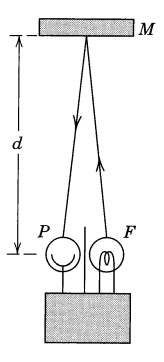
\includegraphics[width=0.2\textwidth]{p1.png} 
\end{center}
Suppose that the clockmoves with a uniform velocity $v$, perpendicular to the
line from $PF$ to $M$, relative to an observer. Using the second postulate of
relativity, show by explicit geometrical or algebraic construction that the
observer sees the relativistic time dilation as the clock moves by.

(b) For simplicity consider just one spatial dimension, and consider a rod
sitting in its rest frame. At $t=0$, one end is at $x=0$ and the other end is at
$x=l$; call these spacetime events $A$ and $B$, respectively. Therefore we say
the rod has length $l$ in its own frame. Now switch to a frame moving at
relative velocity $v$ with coordinates $x',t'$. Spacetime event $A$ is still at
the origin in the new coordinates. Find the location of spacetime event $B$ in
the new coordinates; notice that $x_B'>x_B$, so we might naively conclude the
rod is \textit{longer} in the moving frame, but this is wrong. Explain what is
wrong with this way of measuring the length of the rod.

Instead, measure the length of the rod in the moving frame by sitting at the
origin $x'=0$ and measuring the times $t'$ when the two ends go by. Combined
with the velocity $v$ of the rod, deduce a length $l'$ in the moving frame, and
relate this back to what is seen in the original frame. Show that $l'=l/\gamma$:
in the moving frame, the rod's length is \textit{contracted}.
\begin{solution}
(a) Suppose the observer measures a time period $\Delta t'$ for the clock to
tick when it moves pass them. Then the path that light took was
\begin{equation}
    2L'=c\Delta t', 
\end{equation}
in that period. However, the clock also traverses a distance $v\Delta t'$ during
that period (see figure below).
\begin{center}
    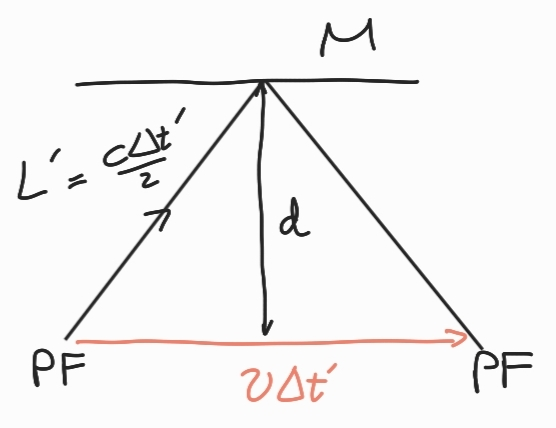
\includegraphics[width=0.4\textwidth]{hw6_p1.jpg} 
\end{center}
Thus, by Pythagorean theorem, we can write
\begin{equation}
    L'^2=\frac{c^2\Delta t'^2}{4}
    =d^2+\frac{v^2\Delta t'^2}{4}.
\end{equation}
Solving for $\Delta t'$, we get
\begin{equation}
    \Delta t'=\frac1{\sqrt{1-\beta^2}}\frac{2d}{c}
    =\gamma\Delta t,
\end{equation}
where $\beta=v/c$. Since $\gamma>1$ because $v<c$ (second postulate), 
$\Delta t'> \Delta t$. So time is dilated for the observer.

(b) By Lorentz transformation, we can write
\begin{equation}
    x_B'=\gamma(-\beta ct+x_B)=\gamma l>x_B, 
\end{equation}
since $t=0$. This way of measuring the length is wrong because the notion of
simultaneity is not preserved under frame transformation. So $A$ and $B$ might
be simultaneous in the rest frame, but not in the moving frame unless $v=0$.

Now, by the inverse Lorentz transformation, for an observer at $x'=0$,
\begin{equation}
    x_A=\gamma(\beta ct_A'+x_A')
    =\gamma vt_A',\qquad\text{and}\qquad
    x_B=\gamma(\beta ct_B'+x_B')
    =\gamma vt_B'.
\end{equation}
Thus,
\begin{equation}
    \Delta t'=t_B'-t_A'=\frac{x_B-x_A}{\gamma v}
    =\frac{l}{\gamma v}.
\end{equation}
The measured length in the observer's frame is $l'=v\Delta t'$ and we get
$l'=l/\gamma$, meaning $l'<l$; the rod is contracted.
\end{solution}
\end{problem}
\newpage
%%%%%%%%%%%%%%%%%%%%%%%%%%%%%%%%%%%%%%%%%%%%%%%%%%%%%%%%%%%%%%%%%%%%%%%%%%%%%%%    
%%%%%%%%%%%%%%%%%%%%%%%%%%%%%%%%%%%%%%%%%%%%%%%%%%%%%%%%%%%%%%%%%%%%%%%%%%%%%%%
\begin{problem}{6.2}[Lorentz transformation]

(a) Prove that two successive Lorentz transformations with velocities $v_1$ and
$v_2$ result in the composition law,
\begin{equation}
    v_\t{tot}=\frac{v_1+v_2}{1+v_1v_2/c^2}. 
\end{equation}
Convince yourself that for $\abs{v_{1,2}}<c$, one always has
$\abs{v_\t{tot}}<c$.

(b) Define the \textit{boost parameter} (also called \textit{rapidity}) $\zeta$
by
\begin{equation}
    v/c\equiv\tanh\zeta, 
\end{equation}
demonstrate that a Lorentz transformation in terms of $\zeta$ takes the form
\begin{equation}
    x'=x\cosh\zeta-ct\sinh\zeta,\qquad ct'=ct\cosh\zeta-x\sinh\zeta. 
\end{equation}

(c) Show that the boost parameter obeys the composition law
\begin{equation}
    \zeta_\t{tot}=\zeta_1+\zeta_2. 
\end{equation}

(d) Demonstrate that the combination $c^2t^2-x^2$ is invariant under a Lorentz
transformation expressed in the boost parameter form.
\begin{solution}
(a) First, the Lorentz transformation can be written as a matrix
\begin{equation}
    L_i=\mqty(\gamma_i&-\beta_i\gamma_i\\-\beta_i\gamma_i&\gamma_i).
\end{equation}
Then the composite transformation is
\begin{equation}
    L=L_2L_1=\mqty(\gamma_1\gamma_2(1+\beta_1\beta_2)&-\gamma_1\gamma_2(\beta_1+\beta_2)\\-\gamma_1\gamma_2(\beta_1+\beta_2)&\gamma_1\gamma_2(1+\beta_1\beta_2)).
\end{equation}
Setting $\gamma_\t{tot}=\gamma_1\gamma_2\qty(1+\beta_1\beta_2)$, then we can 
write $L$ as
\begin{equation}
    L=\mqty(\gamma_\t{tot}&-\beta_\t{tot}\gamma_\t{tot}\\-\beta_\t{tot}\gamma_\t{tot}&\gamma_\t{tot}), 
\end{equation}
where
\begin{equation}\label{p2a:b}
    c\beta_\t{tot}=v_\t{tot}
    =c\frac{\beta_1+\beta_2}{1+\beta_1\beta_2}
    =\frac{v_1+v_2}{1+v_1v_2/c^2}.
\end{equation}

Also, since $\abs{v_{1,2}}<c$, $v_1v_2/c^2<1$ and $v_1+v_2<2c$. So
\begin{equation}
    v_\t{tot}<\frac{2c}{2}=c. 
\end{equation}

(b) Setting $\beta=\tanh\zeta$, then
\begin{equation}
    \gamma=\frac1{\sqrt{1-\beta^2}}=\frac1{\sech\zeta}=\cosh\zeta. 
\end{equation}
Then we can rewrite the Lorentz transformation as
\begin{equation}
    L=\mqty(\gamma&-\gamma\beta\\-\gamma\beta&\gamma)
    =\mqty(\cosh\zeta&-\sinh\zeta\\-\sinh\zeta&\cosh\zeta)
\end{equation}

(c) Using \eqref{p2a:b}, we can write
\begin{align}
    \tanh\zeta_\t{tot}
    &=\frac{\tanh\zeta_1+\tanh\zeta_2}{1+\tanh\zeta_1\tanh\zeta_2}\notag\\
    &=\frac{\frac{\sinh\zeta_1\cosh\zeta_2+\cosh\zeta_1\sinh\zeta_2}{\cosh\zeta_1\cosh\zeta_2}}{\frac{\cosh\zeta_1\cosh\zeta_2+\sinh\zeta_1\sinh\zeta_2}{\cosh\zeta_1\cosh\zeta_2}}\notag\\
    &=\frac{\sinh(\zeta_1+\zeta_2)}{\cosh(\zeta_1+\zeta_2)}\notag\\
    &=\tanh(\zeta_1+\zeta_2).
\end{align}
Then $\zeta_\t{tot}=\zeta_1+\zeta_2$.

(d) Using the Minkowski metric
\begin{equation}
    \eta=\mqty(1&0\\0&-1), 
\end{equation}
we can show that
\begin{align}
    L^T\eta L
    &=\mqty(\cosh\zeta&-\sinh\zeta\\-\sinh\zeta&\cosh\zeta)
    \mqty(\cosh\zeta&-\sinh\zeta\\\sinh\zeta&-\cosh\zeta)\notag\\
                    &=\mqty(\cosh^2\zeta-\sinh^2\zeta&0\\0&\sinh^2\zeta-\cosh^2\zeta)\notag\\
    &=\eta.
\end{align}
Then with $x'^\alpha=L_\beta^\alpha x^\beta$, it follows that
\begin{equation}
    c^2t'^2-x'^2
    =x'^\alpha\eta_{\alpha\beta}x'^\beta
    =x^\gamma L^{\alpha}_{\gamma}\eta_{\alpha\beta}L_{\delta}^\beta x^\delta
    =x^\gamma\eta_{\gamma\delta}x^\delta
    =c^2t^2-x^2.
\end{equation}
So $c^2t^2-x^2$ is invariant under Lorentz transformation expressed in $\zeta$.
\end{solution}
\end{problem}
\newpage
%%%%%%%%%%%%%%%%%%%%%%%%%%%%%%%%%%%%%%%%%%%%%%%%%%%%%%%%%%%%%%%%%%%%%%%%%%%%%%%
\end{document}
